% {\em
% \bit
% \item
% what is the problem
% \item
% what are the applications
% \eit
% }
Today people all around the world use online social networks (OSNs) not only for personal connections but also for entertainment, to share opinions, to read news and inform themselves and to exchange knowledge and information. With their rise in popularity OSNs in the past decade however, they have become a target for abuse by malicious actors who are spamming the network, attempting to scam users, distribute malware, boost a legitimate user's popularity or increase the visibility of certain content. Furthermore with the 2016 United States presidential election the focus has been on social media rather than traditional media for the first time and the concern over widespread \emph{fake news} influencing public opinion as well as social bots pushing state-actor agendas has been growing~\cite{allcott2017social,grinberg2019fake} with some recent research focusing on identifying fake news using data mining methods~\cite{shu2017fake}.

Many OSNs spend a considerable amount of money and time in the form of manual labor on identifying and removing fake accounts. Our goal is to build on previous research and to improve the classification process for more effective and efficient identification of fake accounts. Unlike other approaches which focus only on basic profile features~\cite{cresci2015fame,malhotra2012studying} or temporal patterns in account activity~\cite{chavoshi2017temporal,ferraz2015rsc,gurajala2015fake}, our approach belongs to a category of graph-based approaches to fake account identification.  

Given the directed graph $G=(V,E)$ induced by the social network's structure as well as additional classification features $m_v$ for every $v \in V$, we want to identify all nodes $v \in V$ that are likely to correspond to fake accounts. We call this graph a social graph (figure \ref{fig:social_graph}). For social networks with bidirectional connections i.e. through friend requests an undirected graph may be used to describe the network structure. It is however vital for the classification task that the false-positive rate be kept low as suspensions of legitimate user accounts can degrade the experience enormously.


\begin{figure}
    \centering
    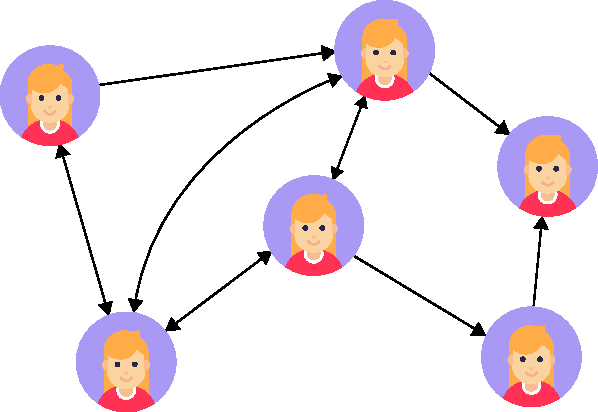
\includegraphics[width=0.4\textwidth]{FIG/social_graph}
    \caption{A social graph}
    \label{fig:social_graph}
\end{figure}


% INCLUDE CONTRIBUTIONS HERE LATER

%The contributions of this project are the following:
%\bit
%\item our proposed {\em someMETHOD} is novel, combining wavelets
%      with a spike-removal  preprocessing step
%\item it is effective, achieving 90\% classification accuracy
%\item it is scalable, being linear on the number of sound-clips $N$.
%\eit

In this paper we propose a novel approach to identification of fake accounts in OSNs by exploiting differences between the ego networks of legitimate users and fake accounts as well as weak links between communities of real users and communities of fake accounts. We first obtain a labelled dataset of legitimate and fake accounts on Twitter. As Twitter's developer policy limits the ways in which scraped user data may be published, these datasets typically contain a list of user IDs which we will then have to scrape to construct the social graph. We will explore this social graph and run experiments to find predictive features based on which we develop a novel approach. Finally, we evaluate our approach in experiments against other popular approaches for fake account detection in OSNs.

The rest of this paper is structured the following way: first we do a short survey of related work and their approaches (Section \ref{sec:survey}), based on the findings in these papers we will explore a dataset of Twitter users and fake accounts and their social graph, propose our own classification method, and evaluate our approach in experiments.